\section{Pol~\abbrsc{III} \abbr{chip}-sequencing quantifies \abbr{trna} gene expression}
\label{sec:chip}

\subsection{\abbr{chipseq} is a \abbr{dna} binding assay}

\define[\defineword{\abbr{chipseq}} \chip followed by high-throughput
sequencing]{\chipseq} is a family of assays based on high-throughput sequencing,
similar to \rnaseq, but pre-dating the latter \citep{Johnson:2007}. Unlike
\rnaseq, which quantifies the abundance of \rna transcripts in the cell,
\chipseq pinpoints loci of protein--\dna interaction for specific proteins that
can be targeted with an antibody. There are several distinct applications of
\chipseq that all rely on the identification and quantification of binding sites
of specific proteins to \dna. The most common uses of \chipseq are
\begin{enumerate*}
    \item the identification of novel \tf binding sites by targeting specific,
        known \tf[s], and
    \item the profiling of histone modifications such as methylation or
        acetylation, which reveal information about the transcriptional activity
        of the proximal sequence (see \cref{sec:transcription})
        \citep{Barski:2007}.
\end{enumerate*}

Briefly, a sample is prepared by cross-linking proteins to the \dna in solution
using formaldehyde to ensure that transient interactions are captured, instead
of being dissolved during the assay preparation. Next, sonication or MNase
treatment is used to shear \dna into smaller fragments. Some of these fragments
will have the protein of interest bound. Using an antibody that recognises the
protein of interest as specifically and sensitively as possible, these fragments
are purified. The protein is then unlinked and the remaining \dna fraction is
again purified, size selected, ligated to sequencing adapters, amplified and
sequenced (\cref{fig:chip-seq-workflow}) \citep{Park:2009}.

\textfig{chip-seq-workflow}{body}{0.5\textwidth}
    {Possible \chipseq workflow.}
    {\todo{Add correct image, explanation}}

\subsection{Quantifying expression of \abbr{trna} genes}

We quantified \trna gene expression via \pol3 \chipseq, using an antibody that
recognises the \pol3 subunit \abbrsc{RPC1/155}, which forms part of the active
centre of \trna gene transcription \citep{Ablasser:2009}. The reason for using
this, on the first glance, indirect measure is because \trna genes are not
identifiable by their sequence alone: performing a multiple sequence alignment
of \trna genes in \mmu reveals that several \trna genes share the exact same
sequence (\cref{fig:trna-alignment}).

\textfloat{trna-alignment}{spill}
    {\footnotesize\begingroup
\let\m\mismatch
\begin{tabular}{@{}ll@{}}
    \toprule
    chr5.trna1044 &  \seq{GTCTCTGTGGCGCAATCGGTtAGCGCGTTCGGCTGTTAACCGAAAG...........GtTGGTGGTTCGAGCCCACCCAGGGACG}\\
    chr3.trna750 &   \seq{GTCTCTGTGGCGCAATCGGTtAGCGCGTTCGGCTGTTAACCGAAAG...........GtTGGTGGTTCGAGCCCACCCAGGGACG}\\
    chr3.trna298 &   \seq{GTCTCTGTGGCGCAATCGGTtAGCGCGTTCGGCTGTTAACCGAAAG...........GtTGGTGGTTCGAGCCCACCCAGGGACG}\\
    chr3.trna294 &   \seq{GTCTCTGTGGCGCAATCGGTtAGCGCGTTCGGCTGTTAACCGAAAG...........GtTGGTGGTTCGAGCCCACCCAGGGACG}\\
    chr3.trna289 &   \seq{GTCTCTGTGGCGCAATCGGTtAGCGCGTTCGGCTGTTAACCGAAAG...........GtTGGTGGTTCGAGCCCACCCAGGGACG}\\
    chr2.trna1947 &  \seq{GTCTCTGTGGCGCAATCGGTtAGCGCGTTCGGCTGTTAACCGAAAG...........GtTGGTGGTTCGAGCCCACCCAGGGACG}\\
    chr1.trna1014 &  \seq{GTCTCTGTGGCGCAATCGGTtAGCGCGTTCGGCTGTTAACCGAAAG...........GtTGGTGGTTCGAGCCCACCCAGGGACG}\\
    chr11.trna1446 & \seq{GTCTCTGTGGCGCAATCGGTtAGCGCGTTCGGCTGTTAACCGAAAG...........GtTGGTGGTTCGAGCCCACCCAGGGACG}\\
    chr10.trna390 &  \seq{GTCTCTGTGGCGCAATCGGTtAGCGCGTTCGGCTGTTAACCGAAAG...........GtTGGTGGTTCGAGCCCACCCAGGGACG}\\
    chr3.trna757 &   \seq{GTCTC\m CGTGGCGCAAT\m CGGT\m cAGCGCGTTCGGCTGTTAACCGAAAG...........GtTGGTGGTTCGAGCCCACCC\m GGGGACG}\\
    chr3.trna283 &   \seq{GTCTCTGTGGCGCAATTGGTtAGCGCGTTCGGCTGTTAACCGAAAG...........GtTGGTGGTTC\m AAGCCCACCCAGGGACG}\\
    \bottomrule
\end{tabular}
\endgroup

    \todo{Fix alignment of table}}
    {Alignment of Asn \trna genes.}
    {Parts of a multiple sequence alignment of \trna genes in \mmu generated
    with COVE\@. Shown are the \trna genes coding for Asn. Bases which differ
    from the consensus sequence are highlighted in red.}

Consequently, to identify individual \trna genes and to quantify their
expression, we cannot use conventional \rnaseq, since the \rna reads covering
only the transcribed gene region are not uniquely mappable. Common strategies
for counting ambiguously mapping reads, as used in \name{ERANGE} by
\citet{Mortazavi:2008}, still require at least \emph{some} unambiguous
information, to distinguish different genes that share reads (and the problem of
multi-mapping reads continues to pose challenges, as recent publications
highlight \citep{Kahles:2015}).

We solve this problem by extending the \trna gene body into the flanking
regions, which are not under purifying selection, and therefore not conserved.
As \pol3 \chipseq fragments cover the flanking regions as well as the actual
gene body (\cref{fig:trna-pol3-binding-profile}), we can use reads uniquely
mapping to the flanking regions to assign ambiguously mapped reads to the
appropriate regions (\cref{fig:trna-pol3-map-ambiguous-reads}).

\textfig{trna-pol3-binding-profile}{body}{\textwidth}
    {\trna \pol3 \chip binding profile.}
    {The shaded, bell-shaped area shows an idealised binding profile of \chipseq
    data spanning the \trna gene with the A and B box highlighted, as well as
    its flanking regions upstream and downstream of the gene body. This overlap
    plays a role in identifying the individual gene.}

More precisely, when mapping the reads, we do not discard all ambiguously
mapping reads. However, we still discard reads which are likely \pcr duplicates,
i.e.\ we remove all but one copy of non-unique reads in the raw input data.
Despite this, we still have reads that have not been uniquely assigned to a
given \trna gene (\cref{fig:trna-pol3-map-a}). To assign these reads, we use the
number of uniquely mapping reads in \trna genes’ flanking regions to determine
the most likely origin (\cref{fig:trna-pol3-map-b}) \citep{Kutter:2011}.

Formally, let \(i\) be the \(i\)th \trna gene locus, and \(c_i\) be the count of
uniquely mapped reads in its flanking region (we used \SI{\pm100}{bp}, which has
been shown to work well in practice \citep{Kutter:2011}). A multi-mapping read
\(r\), which maps to a set \(T\) of candidate \trna[s], can be allocated to a
target \trna gene \(i\) randomly with probability

\begin{equation}
    p_i = \begin{cases}
        c_i \big/ \sum_{x \in T}c_x &
            \text{if \(\sum_{x \in T}c_x \neq 0\),} \\
        1 \big/ \vert T \rvert & \text{otherwise.}
    \end{cases}
\end{equation}

\textfloat{trna-pol3-map-ambiguous-reads}{body}{%
    \centering
    \begingroup
        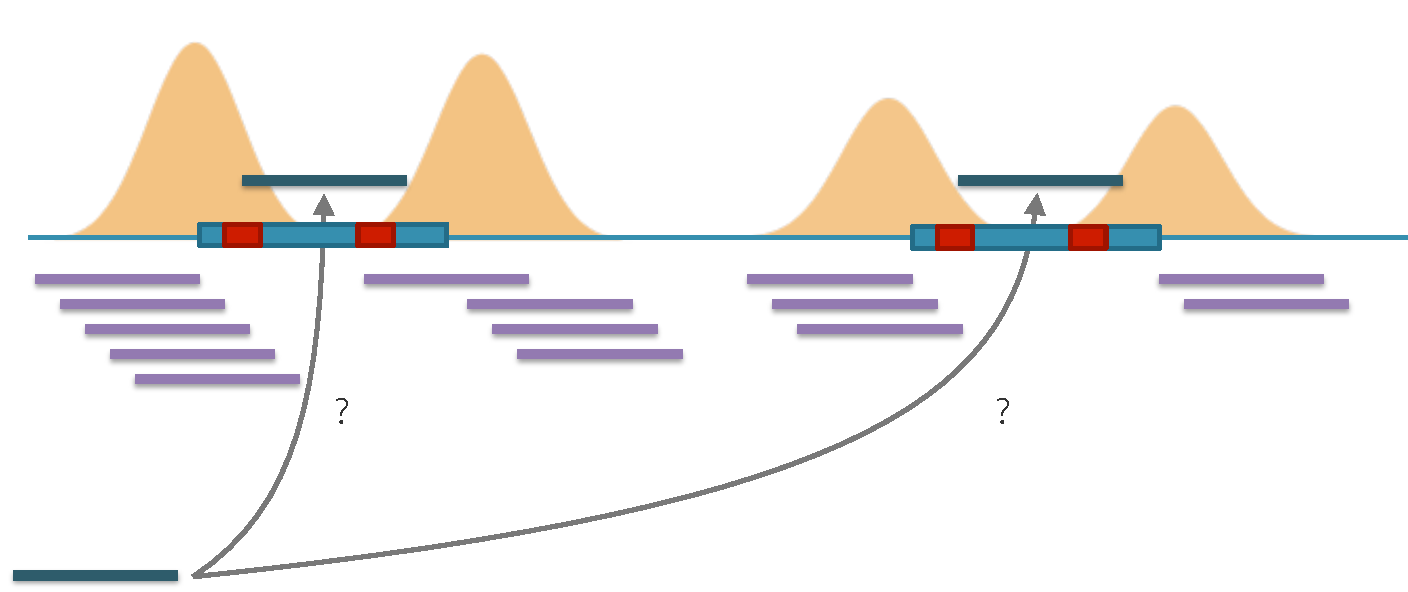
\includegraphics[width=\textwidth]{trna-pol3-map-ambiguous-reads-1}
        \subcaption{\label{fig:trna-pol3-map-a}Two potential match candidate
            \trna genes for a read.}
    \endgroup
    \begingroup
        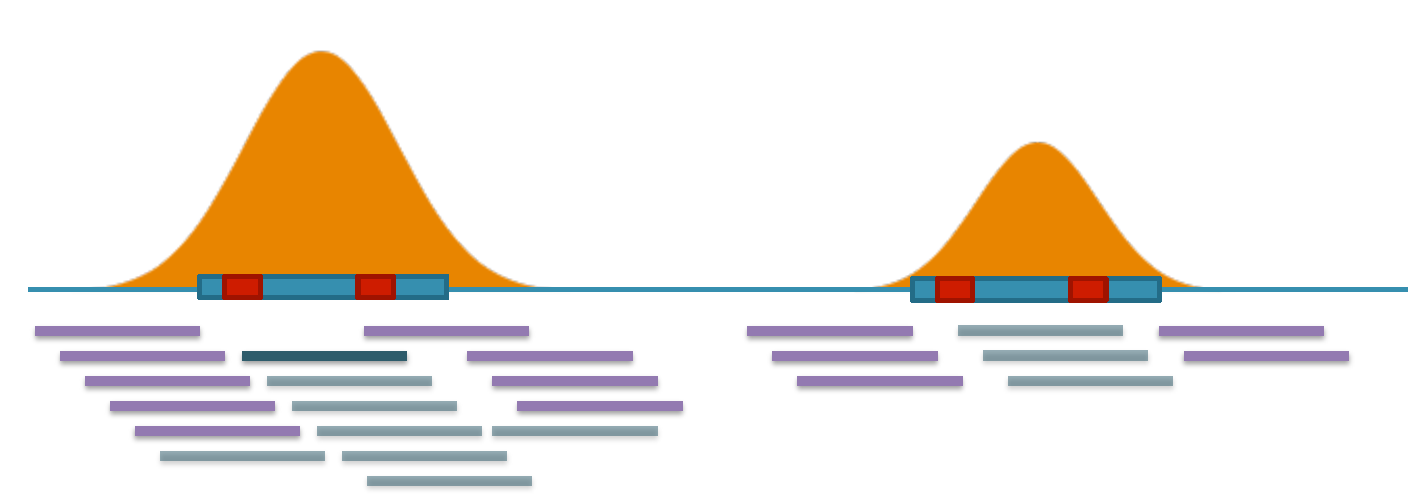
\includegraphics[width=\textwidth]{trna-pol3-map-ambiguous-reads-2}
        \subcaption{\label{fig:trna-pol3-map-b}Using the count data from the
            flanking regions to extrapolate most likely mapping positions for
            ambiguous reads.}
    \endgroup}
    {Mapping ambiguous \chip reads.}
    {\chip reads originating from \trna genes can often not be mapped
    unambiguously to any given \trna. Instead, information form the gene’s
    flanking regions is used to determine the more likely provenance.}
